\documentclass{standalone}
\usepackage{tikz}
\usepackage{ctex,siunitx,ninecolors}
\setCJKmainfont{Noto Serif CJK SC}
\usepackage{tkz-euclide}
\usepackage{amsmath}
\usepackage{wasysym}
\usetikzlibrary{patterns, calc}
\usetikzlibrary {decorations.pathmorphing, decorations.pathreplacing, decorations.shapes}
\begin{document}
\small
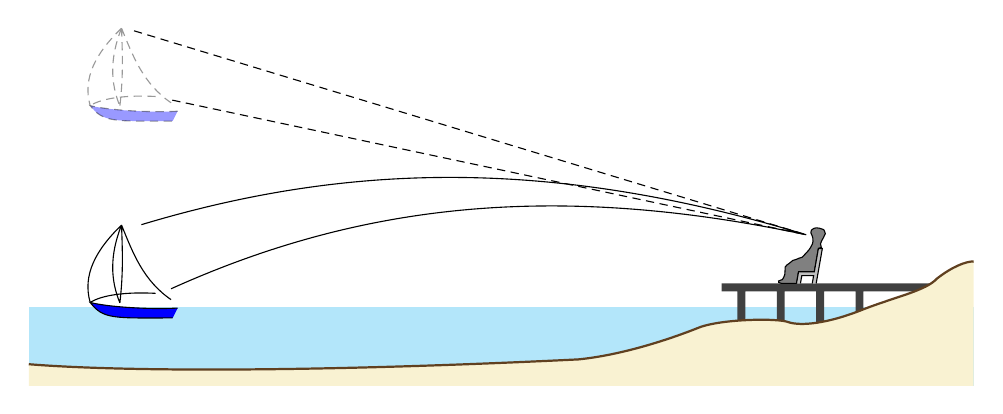
\begin{tikzpicture}[>=latex,scale=1.0]
  \fill[cyan!30](0,0)rectangle(12,1);
  \fill[darkgray](8.8,1.3)rectangle(11.5,1.2)(9,1.2)rectangle(9.1,0)(9.5,1.2)rectangle(9.6,0)(10,1.2)rectangle(10.1,0)(10.5,1.2)rectangle(10.6,0);
  \fill[brown!50!yellow!20](0,0)--( 0.000,0.274)..controls( 1.153,0.180)and( 3.565,0.169)..
  ( 6.979,0.335)..controls( 7.471,0.384)and( 8.030,0.551)..
  ( 8.472,0.724)..controls( 8.755,0.854)and( 9.524,0.860)..
  ( 9.644,0.809)..controls( 9.805,0.755)and(10.147,0.788)..
  (10.607,0.974)..controls(11.026,1.135)and(11.395,1.210)..
  (11.533,1.361)..controls(11.729,1.513)and(11.894,1.578)..(12,1.580)--(12,0)--cycle;
  \draw[brown!50!black,thick]( 0.000,0.274)..controls( 1.153,0.180)and( 3.565,0.169)..
  ( 6.979,0.335)..controls( 7.471,0.384)and( 8.030,0.551)..
  ( 8.472,0.724)..controls( 8.755,0.854)and( 9.524,0.860)..
  ( 9.644,0.809)..controls( 9.805,0.755)and(10.147,0.788)..
  (10.607,0.974)..controls(11.026,1.135)and(11.395,1.210)..
  (11.533,1.361)..controls(11.729,1.513)and(11.894,1.578)..(12,1.580);
  \draw[fill=gray](10.065,1.758)--(10.055,1.803)--(10.071,1.844)--(10.092,1.881)--(10.116,1.932)--(10.104,1.969)--(10.094,1.984)--(10.043,2.001)--(10.003,2.006)--( 9.969,1.999)--( 9.939,1.976)--( 9.932,1.943)--( 9.949,1.904)--( 9.958,1.874)--( 9.959,1.834)--( 9.952,1.801)--( 9.928,1.756)--( 9.908,1.725)--( 9.874,1.688)--( 9.823,1.633)--( 9.782,1.620)--( 9.747,1.605)--( 9.703,1.592)--( 9.659,1.556)--( 9.628,1.534)--( 9.605,1.507)--( 9.605,1.471)--( 9.601,1.412)--( 9.589,1.381)--( 9.571,1.349)--( 9.540,1.338)--( 9.522,1.331)--( 9.523,1.314)--( 9.537,1.308)--( 9.561,1.300)--(9.75,1.3)--++(80:0.15)--++(0.2,0)--++(80:0.3)--cycle;
  \draw[fill=lightgray,even odd rule](9.75,1.3)--++(80:0.15)--++(0.2,0)--++(80:0.3)--++(0.05,0)--++(-100:0.45)(9.8,1.3)--++(80:0.1)--++(0.15,0)--++(-100:0.1);
  \draw(1.807,1.232)..controls(4.163,2.295)and(6.631,2.606)..
  (9.873,1.918)..controls(6.707,2.879)and(4.114,2.855)..(1.430,2.046);
  \draw[densely dashed](1.822,3.628)--(9.873,1.918)--(1.325,4.512);
  \begin{scope}
    \draw[fill=blue](1.890,0.987)..controls(1.519,0.967)and(1.000,1.002)..
    (0.780,1.058)..controls(0.946,0.844)and(1.073,0.860)..(1.828,0.862);
    \draw(1.612,1.174)..controls(1.236,1.194)and(0.930,1.154)..(0.780,1.058)
    (1.178,2.041)..controls(1.195,1.605)and(1.194,1.386)..(1.157,1.053)
    (1.178,2.041)..controls(1.325,1.679)and(1.455,1.336)..(1.807,1.094)
    (1.178,2.041)..controls(0.848,1.723)and(0.680,1.403)..(0.780,1.058)
    (1.178,2.041)..controls(1.028,1.665)and(1.036,1.346)..(1.157,1.053);
  \end{scope}
  \begin{scope}[yshift=2.5cm,densely dashed,opacity=0.4]
    \draw[fill=blue](1.890,0.987)..controls(1.519,0.967)and(1.000,1.002)..
    (0.780,1.058)..controls(0.946,0.844)and(1.073,0.860)..(1.828,0.862);
    \draw(1.612,1.174)..controls(1.236,1.194)and(0.930,1.154)..(0.780,1.058)
    (1.178,2.041)..controls(1.195,1.605)and(1.194,1.386)..(1.157,1.053)
    (1.178,2.041)..controls(1.325,1.679)and(1.455,1.336)..(1.807,1.094)
    (1.178,2.041)..controls(0.848,1.723)and(0.680,1.403)..(0.780,1.058)
    (1.178,2.041)..controls(1.028,1.665)and(1.036,1.346)..(1.157,1.053);
  \end{scope}
\end{tikzpicture}
\end{document}